\documentclass[10pt,a4paper]{article}
\usepackage[utf8]{inputenc}
\usepackage[T1]{fontenc}
\usepackage{lmodern}
\usepackage[margin=1.5cm, top=1.4cm, bottom=1.4cm]{geometry}
\usepackage{hyperref}
\usepackage{enumitem}
\usepackage{titlesec}
\usepackage{xcolor}
\usepackage{graphicx}

\definecolor{accent}{HTML}{00686E}
\hypersetup{colorlinks=true, urlcolor=accent, linkcolor=accent}
\pagenumbering{arabic}
\setlength{\parindent}{0pt}

\titleformat{\section}{\large\bfseries\color{accent}}{}{0em}{}[\vspace{-0.6em}\rule{\textwidth}{0.8pt}]
\titlespacing{\section}{0pt}{7pt}{4pt}

\newcommand{\role}[4]{%
  \textbf{#1} \hfill \textbf{#2}\\[1pt]%
  \textit{#3} \hfill \textit{#4}\\[2pt]%
}
\setlist[itemize]{leftmargin=1.2em, itemsep=1.5pt, topsep=2pt, parsep=0pt}

\begin{document}

% ================= HEADER =================
\begin{minipage}[c]{0.80\textwidth}
  {\Huge\bfseries Prabhavit Gupta}\\[3pt]
  {\color{accent}\large AI Engineer: Production LLM Pipelines, MCP Tooling \& Automated Evaluation}\\[6pt]
  {\footnotesize +39 351 610 7807 ~$\vert$~
  \href{mailto:prabhavitg@gmail.com}{prabhavitg@gmail.com} ~$\vert$~
  \href{https://www.linkedin.com/in/prabhavit/}{linkedin.com/in/prabhavit} ~$\vert$~
  \href{https://github.com/prab-gupta}{github.com/prab-gupta} ~$\vert$~
  Venice, Italy}
\end{minipage}\hfill
\begin{minipage}[c]{0.18\textwidth}
  \raggedleft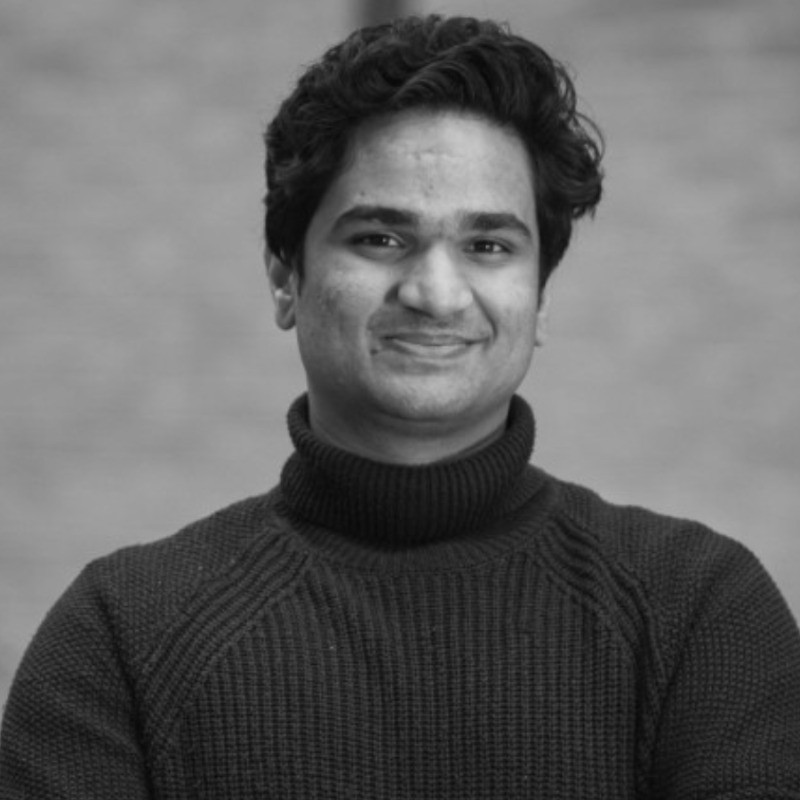
\includegraphics[width=2.0cm]{photo.jpg}
\end{minipage}
\vspace{-2pt}

% ================= SUMMARY =================
\section{Summary}
AI Engineer and Automation Developer with 3 years of hands-on experience designing, developing, and shipping production ML/LLM systems, intelligent data pipelines, and agent architectures. Expert in building Python-based data ingestion and classification pipelines, integrating disparate models and databases (PostgreSQL, Supabase), and architecting custom MCP (Model Context Protocol) servers and tooling. Proven track record deploying automated evaluation frameworks and rigorous end-to-end testing suites to validate model accuracy, latency, and reliability on live customer data. Experienced collaborating across engineering and product teams to translate ambiguous business requirements into robust, high-impact AI features. Based in Venice, Italy with an EU Long Term Residence Permit (unrestricted EU work authorization without visa sponsorship). Immediately available.

% ================= TECHNICAL EXPERTISE =================
\section{Technical Expertise}
\begin{itemize}
  \item \textbf{AI \& LLM Systems:} Production LLM pipelines, Prompt engineering, Structured JSON outputs, Function calling, Multi-label classification, RAG architectures, LLM inference optimization, Context caching.
  \item \textbf{MCP \& Tooling Development:} Building, maintaining, and extending MCP (Model Context Protocol) servers and connectors, API integrations, Agent tooling workflows, Claude Code daily power-user.
  \item \textbf{Languages \& Frameworks:} Python (data processing, API integration, pipeline automation), TypeScript, JavaScript, Node.js, SQL, Next.js, Shell scripting, Git.
  \item \textbf{Data Stores \& Processing:} PostgreSQL, Supabase, Relational schema design, Query optimization, Vector embeddings, Web scraping \& data extraction pipelines.
  \item \textbf{Evaluation \& Testing:} Automated testing frameworks (Playwright, Postman), System verification, Continuous integration, Error diagnostics, Data quality monitoring.
  \item \textbf{Languages \& Work Authorization:} Hindi (Native), English (C1 Professional), Italian (Beginner). EU Long Term Residence Permit (Permanent unrestricted work authorization in Italy and EU without visa sponsorship).
\end{itemize}

% ================= EXPERIENCE =================
\section{Experience}

\role{\href{https://flowspace.co}{FlowSpace.co}}{Mar 2024 - Aug 2026}{Lead Developer (Full-time, Freelance)}{London, UK (remote)}
\begin{itemize}
  \item Built and deployed custom LLM pipelines and automated ingestion workflows in Python, extracting structured attributes from unstructured data sources and populating 900+ active partner listings.
  \item Designed and stood up automated end-to-end testing suites with Playwright, systematically validating pipeline execution, API contract compliance, and model output stability.
  \item Developed and integrated internal MCP tooling and API connectors connecting operational platforms (OfficeRnD, Nexudus, CRM) to enable autonomous agent execution.
  \item Engineered AI-assisted customer triage agents using Claude API with strict schema validation, cutting repetitive support ticket volume.
  \item Oversaw platform migration from a legacy stack to a modern Next.js and Laravel architecture, scaling active user capacity from 2,000 to 4,500+ users.
  \item Diagnosed and resolved live data inconsistencies and pipeline bottlenecks reported by enterprise stakeholders, maintaining high data fidelity.
  \item Leveraged Claude Code daily to compress iteration cycles and deliver production-ready features rapidly.
\end{itemize}

\role{Urlink}{Apr 2025 - Jul 2025}{Project Manager \& AI Assisted Developer (Freelance)}{Barcelona, Spain (remote)}
\begin{itemize}
  \item Directed delivery of core application features, establishing database schemas, API contracts, and data transformation scripts in relational environments.
  \item Built automated backend data validation pipelines connecting third-party services with PostgreSQL, preventing malformed inputs and ensuring zero data loss.
  \item Set up CI/CD workflows and regression testing to maintain deployment reliability and application performance.
\end{itemize}

\role{Independent Technical Consultant}{Aug 2023 - Feb 2024}{AI Solutions \& Automation Engineer}{Venice, Italy}
\begin{itemize}
  \item Developed bespoke AI workflows, automated web extraction engines, and API connectors for European SME clients using Python and TypeScript.
  \item Analyzed operational bottlenecks across customer-facing workflows, architecting and shipping automated tools that eliminated manual data entry.
  \item Built real-time webhook consumers and database synchronization tools with automated error handling and logging.
\end{itemize}

% ================= EDUCATION =================
\section{Education}
\role{Ca' Foscari University of Venice}{2020 - 2024}{BA in Philosophy, International Studies and Economics}{Venice, Italy}
\begin{itemize}
  \item Rigorous foundation in formal logic, analytical problem solving, systems analysis, and macroeconomic decision models.
\end{itemize}

\end{document}
